\section{Introduction}
In this short tutorial you will get a brief overview over Moflon. We show you some features in some little examples. When you have finished this tutorial, you will have an idea what you can do with this tool.
\newline
But first we recomend that you work through Part I for installation instructions.

\subsection{Seting up your workspace}
If you have worked through Part I, you can skip this chapter and go on with the next one. Otherwise open the \texttt{Install, configure and deploy Moflon} button, go to \texttt{Install Workspace} and select the \texttt{Demo Workspace} (Fig.~\ref{demo_workspace}). Now you have all necessary files to work through this tutorial.

\begin{figure}[htbp]
	\centering
  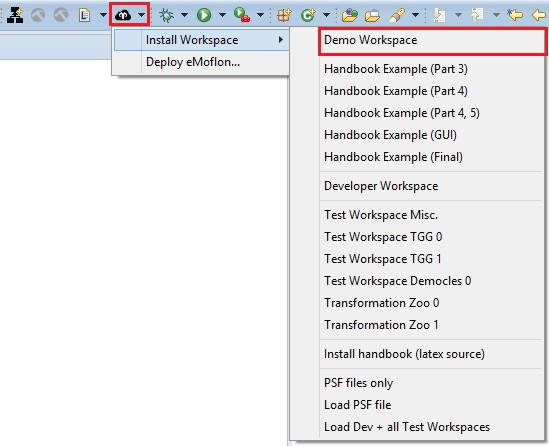
\includegraphics[width=1\textwidth]{eclipse_MoflonButton}
	\caption{Check out of the Demo Workspace} 
	\label{demo_workspace} 
\end{figure}